\begin{table} 
\begin{center} 
\begin{tabular}{|c||c|c|c|c|}
\hline
\emph{Algorithm} & \emph{Manifold Model} & \emph{Encode} & \emph{Decode} & \emph{Relate Enc. \& Dec.}\\
%\thickhline
\hline \hline 
\cellcolor{red}PCA & Linear &\checkmark & \checkmark & $W_D = W_E ^T$\\
\hline
\cellcolor{red}ICA & Linear &\checkmark & \checkmark & $W_D = W_E ^T$\\
\hline
\cellcolor{yellow}Sparse Coding & Local Linear &\checkmark & \checkmark & Separate \\
\hline 
\cellcolor{yellow}PSD \& LISTA & Local Linear &\checkmark & \checkmark & Separate\\
\hline
\cellcolor{lightblue}DrLIM & Nonlinear & \checkmark & X & Enc. Only\\
\hline
\cellcolor{lightblue}Chapter \ref{chapter:slow} & Nonlinear & \checkmark & X & Enc. Only\\
\hline
\cellcolor{lightblue}Chapter \ref{chapter:linear} & Nonlinear & \checkmark & \checkmark & Separate\\
\hline
Adversarial Networks & Nonlinear & X & \checkmark & Dec. Only \\
\hline 
\cellcolor{green}Auto-Encoders & Nonlinear & \checkmark & \checkmark & Separate \\
\hline 
\end{tabular} \\
\vspace{0.25cm} \hspace{0.25cm}  
\begin{tabular}{|c|}
\hline 
\emph{Model Objective/Prior}\\  
\hline \hline
\cellcolor{red} De-correlation/Independence  \\
\hline
\cellcolor{yellow} Sparsity \\
\hline
\cellcolor{lightblue} Metric Learning/Geometric Prior  \\
\hline
\cellcolor{green} All of the Above \\
\hline
None \\
\hline
\end{tabular}
\end{center}
\caption{Summary of unsupervised feature learning algorithms and their properties} 
\label{tbl:models} 
\end{table} 

Unsupervised feature learning arguably dates back to the invention of Principal
Component Analysis (PCA) in 1901 by Karl Pearson \cite{PCA}. As mentioned in
Chapter \ref{chapter:introduction}, feature learning algorithms model
intrinsically low dimensional data embedded in a high dimensional ambient
space. These models can usually be decomposed into two parts: a mapping from
the input space to the feature space, called encoding, and mapping the feature
space back to the input space, called decoding. If the encoding or decoding
processes have corresponding functional forms, they are referred to as the
``encoder'' and ``decoder'', respectively.  From the natural image manifold
perspective, ideal encodings map the extrinsic coordinates (i.e. pixel values)
to intrinsic manifold coordinates. It is hoped that these intrinsic coordinates
correspond to physical attributes of the natural world, such as the presence of
certain objects in the scene, their properties, etc \cite{nair2008,capsules}.
Unsupervised feature learning models are mainly distinguished by: i-the
geometrical prior they assume about the data manifold, ii-whether they learn an
encoder, decoder, or both. For example, Principal Component Analysis assumes
that the data is concentrated around a hyper-plane, i.e. it assumes a globally
linear data manifold model. The PCA encoder is a matrix operator, $W_e$, as is
the decoder $W_d=W_e^T$.  Obtaining ``invariant'' representations has been a
major driving force in feature learning, driven mainly by recognition and
classification problems.  Invariant features imply that the encoding process is
necessarily a many-to-one mapping. This means that the decoding process must
involve some random selection among the possible inputs that produced the code,
usually  by sampling from a distribution. Models that include a decoder are
called ``generative models'' in the literature. 

Table \ref{tbl:models} summarizes key aspects of several well-known feature
learning models, as well as the new models which will be introduced in Chapters
\ref{chapter:slow} and \ref{chapter:linear}. The first column lists the name of
the model, the color indicates the type of objective each model tries to
optimize.  These are summarized in the table below. For example, one version of
PCA finds maximally decorrelated linear components. The ``manifold model''
column indicates the geometric prior each model assumes about the data
manifold. The next two columns indicate whether each model learns an encoder
and/or decoder.  Finally, the last column summarizes the relationship enforced
between the encoder and decoder. For example in PCA the encoder and decoder are
related by the transpose operator. This chapter will review the algorithms in
Table \ref{tbl:models}, placing emphasis on the precursors of the algorithms
presented in Chapters \ref{chapter:slow} and \ref{chapter:linear}. The
algorithms will be presented as various models of the data manifold.

\section{Principal and Independent Component Analysis} 

\begin{figure} 
\centering
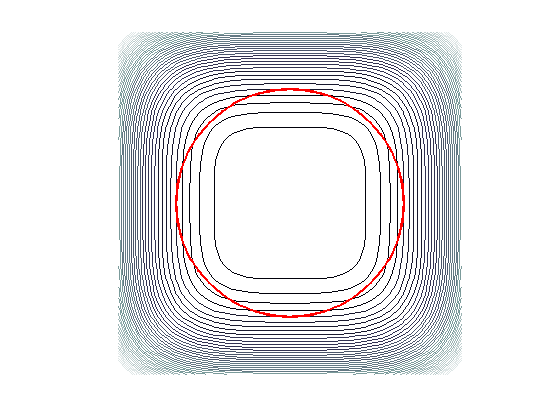
\includegraphics[scale=0.4]{./figures/related_work/ICA.png} 
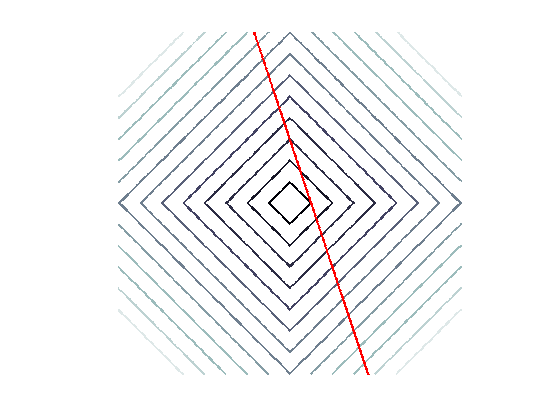
\includegraphics[scale=0.4]{./figures/related_work/L1.png} 
\caption{Left: visualization of the optimization problem used to solve for independent representations. Right: visualization of the optimization problem used to solve for sparse representations.} 
\label{fig:ICA_lasso} 
\end{figure}  

Principal Component Analysis (PCA) and Independent Component Analysis (ICA) are
the most well know linear manifold models \cite{ICA}. Both assume that the
observed high dimensional data $x$ are generated from some low dimensional
latent variables $z$ via a linear operator $A$, that is $x=Az$. Assuming that
the data is zero mean, PCA implicitly makes the assumption that the latent
variables correspond to directions with the largest variance \cite{PCA}. ICA
however searches for linearly independent components, formulating the
definition of independence using the central limit theorem. Although the
detailed derivation of ICA will not be presented here, we will mention that it
leads to a fourth order moment (kurtosis) maximization problem subject to a
second order moment (variance) constraint. This optimization problem is
visualized as the left plot of Figure \ref{fig:ICA_lasso}. The blue curves
represent the level sets of the kurtosis objective, and the red curve
represents the unit variance constraint. 


\section{Sparse Representations} 
Sparse inference refers to the problem of finding the coefficients $z$ which
reconstruct the input $x$ as a sparse linear combination of some basis elements
contained an over-complete dictionary $W_d$. In general, sparse inference is an
intractable combinatorial problem. A relaxation of the sparse inference problem
is the so called lasso, 

\begin{equation} L_{lasso} = \min_Z \frac{1}{2}\|X-W_dZ\| + \alpha |Z|_1
\end{equation} 

\section{Metric Learning}

\section{Regularized Auto-Encoders} 
 
